\chapter{背景综述}

高性能计算(High Performance Computing)一直是计算机科研领域的重要主题。伴随近20年来超级计算集群
性能和数量的指数式增长,我们的超算能力已经迈进Petaflop时代($10^{15}$次浮点运算), 更强大的
exaflop时代($10^{18}$次浮点运算)也即将到来。但是目前能够有效充分利用超算集群的应用程序还为数
不多,因此超算应用是制约HPC界发展的一大瓶颈。\par
在超算的应用领域,科研活动占据了一大部分,如天文学,粒子物理,计算化学等基础学科;另外在工程和
商业领域也有重要的应用,如汽车,飞机设计中得计算流体力学模拟仿真,油田勘探中的海量信息处理和开采
方案设计以及在商业投资领域的高频交易等。此外随着云计算和大数据相关研究和商业应用的快速崛起,
怎样将高性能计算和数据挖掘分析等技术结合起来也成为了当前超算领域的研究热点。本文的主题是探讨
高性能计算在金融领域的一个重要应用以及其在Intel最新的MIC架构上的实现。首先在中我们将简单介绍
高性能计算和金融领域超算应用的一些基本情况。

\section{高性能计算的诞生和发展} % (fold)
\label{sec:intro-hpc}

高性能计算的概念和实现依赖于算法理论和硬件制造的发展。在算法理论方面,并行运算(Parallel computing)
的研究在70年代就开始,但是受制于当时硬件领域的发展瓶颈,并行运算方面的很多理论没有得到充分地发展。
如图\ref{fig:intelProcessor} 所示,Intel的处理器的在2000年之前晶体管的数量和时钟频率都能依照摩尔定律增长。
\begin{figure}
	\centering
	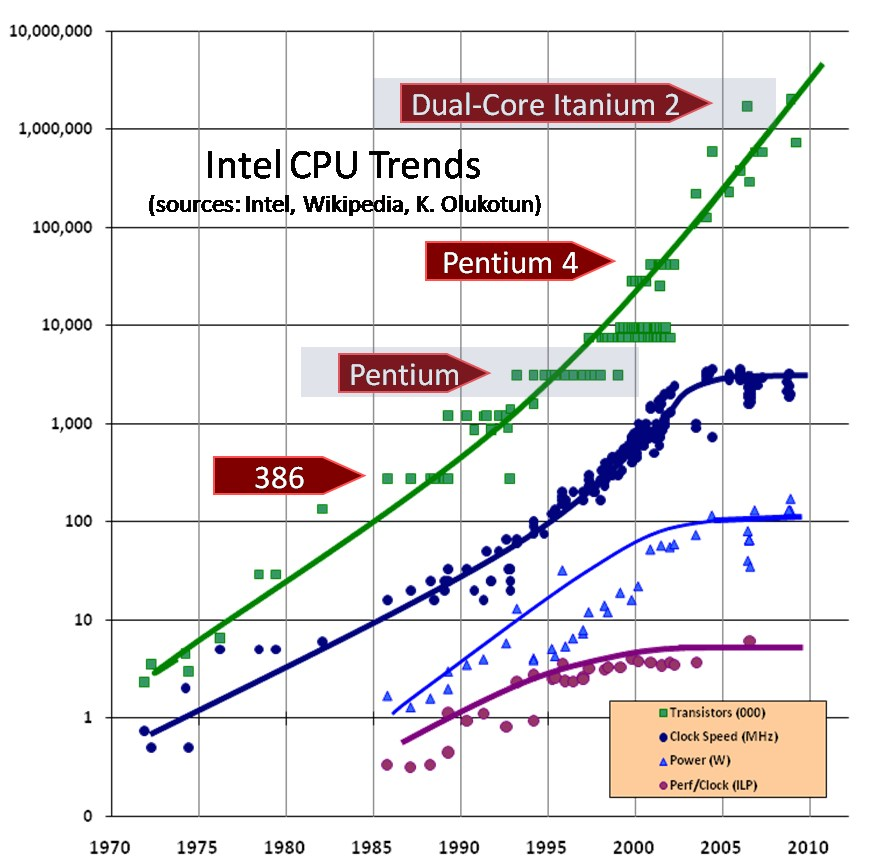
\includegraphics[width=\textwidth]{chap1/Figures/CPU-Scaling.jpg}
	\caption{Intel处理器的发展趋势}
	\label{fig:intelProcessor}
\end{figure}
但是当单个处理器的制造工艺到达纳米级别后,受制于量子效应已经无法进一步提高单个处理器的时钟频率。
随后业界开始转而使用多核系统(Multi-core system),直至目前出现的众核系统(Manycore system)来提升超算的性能。目前最权威的HPC超算
集群排行榜Top500给出的结果显示,无论是排名第一的机器还是所有500强计算能力的综合都较好地符合摩尔定律逐年增长。
\begin{figure}
	\centering
	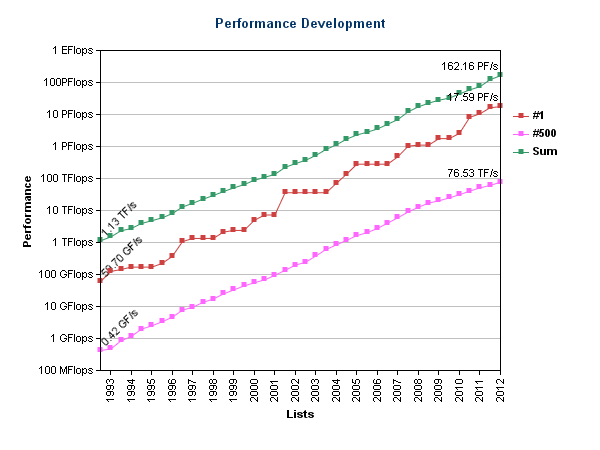
\includegraphics[width=\textwidth]{chap1/Figures/top500Perf.png}
	\caption{Top500超算集群的性能发展}
	\label{fig:top500Perf}
\end{figure}
但是这些峰值运算速度仅仅代表了理论上一台超算集群能够达到的速度,其测试结果也是通过相对简单地基准程序(benchmark)获得的,而真正复杂的应用程序大多数
还未能在超算集群上跑出好的使用效率。制约在超算上展开大规模应用的因素有以下几点。
\begin{enumerate}
    \item 缺少能极大地提供并行性的算法
	\item 数据间的通信受制于内存读取速度和处理器间的连接速度。
	\item 从串行编程模型转到并行编程的学习成本
\end{enumerate}
算法的并行性是最为重要的一点,目前的大多数数学模型和对应的算法没有足够的并行性能够充分发挥超算集群的潜力。我们需要的是面向并行建立新的数学模型和
算法来解决实际问题。同时我们的编程模型和编程语言也需要相应地升级,使之能更自然和原生地支持并行架构。这一点也被认为是同向Exascale计算的关键。
而对于第二点,目前出现的CPU/coprocessor架构已经迈出了重要的一步。Nvidia公司的GPU和GPGPU编程模型可以充分利用GPU的充足带宽(bandwidth)优化数据并行性德问题
(Data Parallel, SIMD),而Intel公司则相应地推出了自己的协处理器Xeon Phi (Many Integrated Core Architecture, MIC Architecture)。Xeon Phi同样拥有强大的
带宽(382G/s)。此外Xeon Phi在编程难度上相比于GPGPU更有利于初学者掌握,实际上用户可以相对简单地从CPU的串行程序过渡到Xeon Phi的并行代码上。
本课题的应用即在MIC架构上展开,并在数据通信等方面进行优化。

% section 高兴能计算的产生和发展 (end)

\section{金融领域的超算应用} % (fold)
\label{sec:intro-finance}
当前的高性能计算在金融领域里的应用有如下几个方面:
\begin{enumerate}
\item 高频交易 
\item 风险管理 
\item 金融衍生品的定价 
\item 定量经济分析 
\end{enumerate}
金融交易借助高性能计算能获得相对的竞争优势,同时也能降低交易风险。2007-2008 次贷危机的主要原因就是所用的金融工具,如担保债务凭证(CDO) 的风险
没有得到正确的认识。而造成这一误判的一个重要原因是模型中用来表示风险参数算法过于复杂,传统的计算机技术对此不能很快得到结果。
从这个角度来说,高性能计算在金融中起着积极的作用因而高性能计算在金融中也越来越重要。

以高频交易为例,其所涉及的IT技术分成三部分:
\begin{itemize}
\item 交易数据在电脑外的加速,就是如何快速地把交易数据(主要是实时行情数据和订单信息),联接和推送到运行程序化交易策略的电脑。
\item 交易数据在电脑内的加速,即如何在电脑内部把交易数据最快地传到交易策略程序。
\item 其他数据的逻辑调用。其他数据主要是指历史行情数据、基本面方面的信息数据以及统计信息等。
      简言之,就是如何快速地获取程序化交易策略下单逻辑所需要的其他判断数据。
\end{itemize}	 
交易数据在电脑外的加速基本上是个花钱的活,美国许多交易所已经实现了co-location 的业务,客户可以花钱把行情服务器、策略服务器等机器放在
交易所撮合引擎服务器所在的数据中心里。从物理距离上来说没有比这更近了。交易所提供的数据支持 主要以1G 和10G以太网接口为主,
10G的比1G网络带宽更大更快,当然也更贵些。随着数据量的增加,以后也会应用40G的InfiniBand 以及更快的以太网。交易数据从交易所出来后,
下面便是交易公司如何部署自己的路由器和交换机了,在这方面也有一些提供高速路由器和交换机的公司,
这些器材 在网络延迟和速度上要比通用的设备要好很多,当然价格也高了不少。
	  
如果程序化交易策略只交易一个品种,在一个交易所co-location就可以满足要求了,但如果策略需要做多个品种,例如期现套利,这就要涉及到两个数据中心的连接。
美国期货的交易重镇主要在中西部的芝加哥,股票现货交易主要在东北部的纽约,由于光速是固定的,两点之间直线最短,谁的光纤最直,谁的物理连接距离最短,
谁的速度就最快。美国有家专门的网络提供商叫Spread Networks,它花了两年铺了纽约和芝加哥目前为止最直的一条网络,
网络连接往返速度只需 13.33毫秒(ms,千分之一秒),比原来的网络少了3毫秒。还有家叫Mckay Brothers的公司,它宣布自己的无线网络可以达到更快的速度。
	   
交易数据从网络传到了电脑后,具体说是到了网卡的网端后,下一步的工作便是把数据传递到交易策略程序了。一般交易策略程序是作为操作系统的用户程序存在。
交易数据主要通过UDP与TCP两种方式进行网络传输,下面以UDP包为例,(TCP 更复杂些,但原理差不多),简单来介绍下交易数据在电脑内的传输、解析。
交易数据到达网卡后,通过PCI Express 或HyperPort接口,再传到操作系统的内核(OS Kernel)进行TCP/IP 协议栈的解析,再把解析后的数据内容通过socket 接口,
推送到用户程序即策略中。然后用户程序再对数据按照规定的格式进行解析,然后应用在策略逻辑中,进行分析,下单等动作。
以上的这种方式主要是基于现有电脑的结构的基本做法,配置好的快些,但总的来说整个过程的处理时间,数量级在两位数微秒(us,百万分之一秒)左右。
数据量多的时候,操作系统内核 对TCP/IP 的解析所用CPU也消耗很多,处理速度会加速下降。一般来说,1G 的数据需要一个GHZ的CPU进行解析,
一般的CPU的速度也就是2-3GHZ,这个比例在数据量大时是相当大的。在整个交易数据内部传递与解析的过程中,能够做文章的主要是TCP/IP 协议的解析和业务数据的解析
。因为策略逻辑的多样性,对策略逻辑的普遍加速的可能性不大。 TCP/IP 协议的解析(TOE,TCP/IPoffload engine)和业务数据的解析主要由专用的网卡来做。
目前有两种方法来实现,一种是在网卡附带的CPU上进行处理,(IBM有一款网卡附带CELL芯 片,也就是SONY在PS3游戏机上用的,功能很强大);
另一种是网卡+FPGA的形式,用FPGA(现场可编辑门阵列)来做TCP/IP的解析和业务数 据的解析。 FPGA 因为全部是硬件,速度会更快些。
理论上来说,用ASIC(专用集成电路)会更快些,但是这个市场是个小众市场,用ASIC并不划算,目前还没有人这么做。 
通过以上的这些硬件加速的方法,基本上能达到个位数微秒(us)的延迟。用硬件做的好处除了延迟小外,在处理的容量上也有诸多好处。
硬件能够做到无论在数据多少都达到固定的性能, 这是基于电脑操作系统结构没法做到的。
	    
交易数据传递、解析在电脑外部的通道和内部的通道都打通后,剩下的便是对程序化交易策略的分析了。由于交易策略的千奇百怪,也无法有一个统一的模式,
就技术难点来说,主要是对大量数据的分析,尤其是对大量时间序列数据的保存和快速访问。
一般的通用办法是用平面文件或者关系型的数据库如ORACLE, MY SQL, SQL Server。这种办法主要瓶颈在于磁盘硬碟的读写的IO速度上。
现在有些基于内存的数据库(In-memory database),可以大大加快读写速度。现在内存的价格下降很快,In-memory database 也越来越可行,但是数据多的话,
还是会有局限。另外,时间序列数据也有其特殊性,它更适合基于列的操作,而通常的数据库系统都是基于行的操作。
在这方面, 也有厂家如KDB 提供专门为海量数据基于列数据库管理系统。
		 
另外,高频交易所用的其它周边系统还有信息传输系统(Messaging System),它主要是来传递各个子系统间的信息传送;还有数据储存系统,
它主要是来保存每天产生的海量数据以及这些数据的读写。现在如果单单把美国股 票市场的数据保存,每天需要超过100G,一个月超过2T。
如果要保存多市场多品种的数据,数据量更是惊人。一个好的高频交易平台也包括良好的回测复盘工具,用以有效率地开发调试策略。
一天100G的数据跑下来,用平常的方法效率太慢,如果要跑多天的话,更是慢得没法接受。另外,模拟成交也是一个大问题, 尤其在超高频的情况下。
		  
以s上即高频交易中的主要技术问题。 其实许多高频的交易的做法和思路都比较公开,很多高频交易策略也大都大同小异。所以一个成功的高频交易策略,
除了在交易算法和细节处理之外,更多的是在于他所使用的交易系统的处理能力和速度上。确切的说,高频策略的成功与否,
很大程度上取决于能否在众多竞争者中抢到自己要的单子。在美国,高频交易者往往需要花大钱搭建交易网络和购买最好的硬件,使自己能够得到最快的数据和交易通道。
同时,他还要不停地跟踪策略的交易情况,调整策略算法逻辑,不断地跟踪策略对行情的反应时间、下单的速度以及交易延迟的情况,
试着把策略的反应时间再缩短1微秒。
% section 金融领域的超算应用 (end)


